\chapter{Results of the simulation}
\section{Statistics and gathered results}

During the testing phase of the app we have gathered more than 8000 location records that had to be filtered and ran through our algorithm. We have made a total of 21 paths with walking, bus riding and car driving. During testing, we have tweaked the algorithm for it to show as accurate results, as possible. We think, the app performs alright, but the accuracy of the GPS signal could be improved.

\section{Algorithm calibration and data validation}

During the development phase we have picked 9 km/h as a maximum of human walking speed and set that as a limit. After making a few passes and trying the app out, we have found 9 km/h to be not enough, as it removes any kind of running and does not take into consideration GPS inaccuracy. What we have discovered, is that if someone moved 12 meters, which makes it a plausible distance to be walked in as depicted in the equation \ref{eq:distancespeed}, GPS inaccuracy made that distance to be 14 meters, which removed the readout.
\begin{equation} \label{eq:distancespeed}
    t = 5[s];~~ x = 12[m];~~ \bar{v} = \frac{\Delta x}{\Delta t} = \frac{12}{5} [\frac{m}{s}] = 2.4 [\frac{m}{s}] = 7.2 [\frac{km}{h}] < 9 [\frac{km}{h}]
\end{equation}
After some testing, we have found 20 km/h to be an optimal value. It does not exclude runners, but does correctly filter any car driving, as we have found a 30 km/h to be a minimum value a car moves in, even when going through speed bumps. The only exception is a standstill or a very slowly moving traffic jam. Our algorithm does filter out any standstill, but cannot handle a very slowly moving car. It would be invalid to assume someone is in a slowly moving car, as it is very possible they are walking at that moment. Perhaps a look at a larger picture, taking into consideration more context would help, but machine learning could be a valid solution as well.

\section{Comparison of the results with real data}

We have put a lot of time to validate data and polish the algorithm to give the best results possible. In the following subsections, there are a few examples presented. They should give the reader a whole picture on how the app works and what is happening behind the scenes.

\begin{figure}[]
    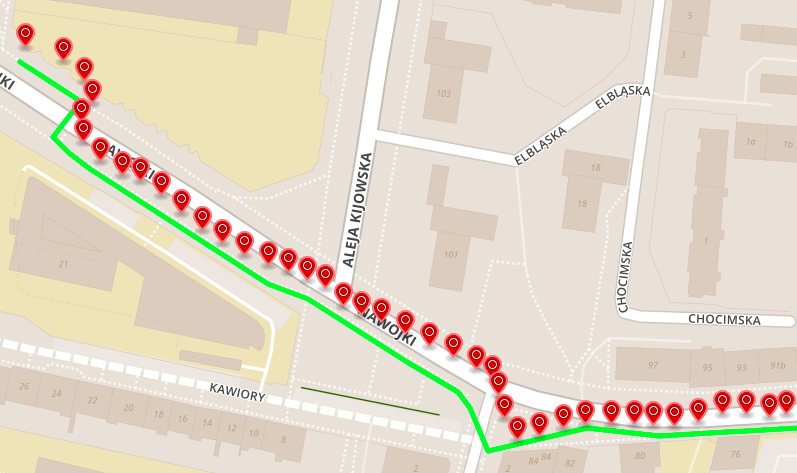
\includegraphics[width=0.9\textwidth]{images/1.png}
    \caption{Green path is the actual path, red pins depict non-filtered readouts. \\ \textit{source: own elaboration}}
    \label{fig:screenexample1}
\end{figure}

\subsection{Example 1: Accurate walking readouts}

This is an example, when readouts during walking are correctly read and displayed on the map. As can be seen in the figure \ref{fig:screenexample1}, presented location differs from actual position a little due to GPS inaccuracy. This inaccuracy is not substantial and is not a subject of this work.

\begin{figure}[]
    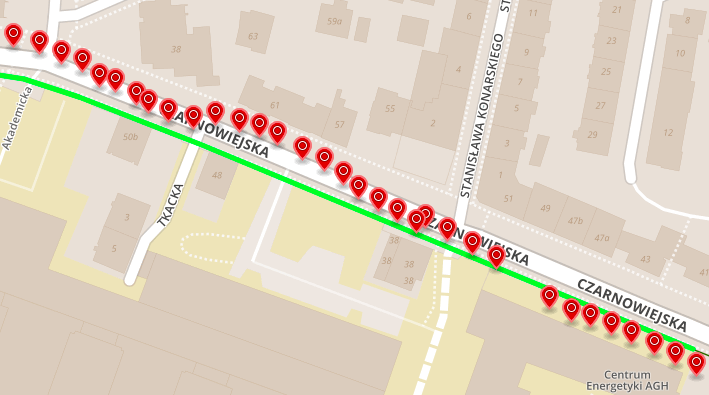
\includegraphics[width=0.9\textwidth]{images/1-1.png}
    \caption{Green path is the actual path, red pins depict non-filtered readouts. \\ \textit{source: own elaboration}}
    \label{fig:screenexample11}
\end{figure}

\begin{figure}[]
    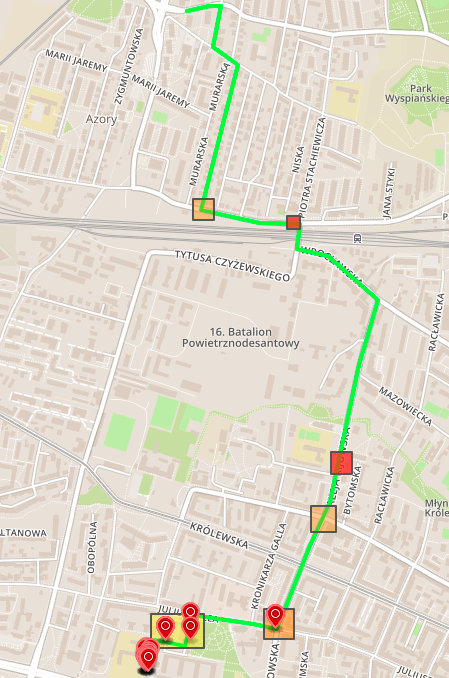
\includegraphics[width=0.9\textwidth]{images/2.png}
    \caption{Green path is the actual path, red pins depict non-filtered readouts, red boxes mean stoppage points, orange boxes depict areas of real slowdowns, yellow area shows a very slow movement. \\ \textit{source: own elaboration}}
    \label{fig:screenexample2}
\end{figure}

\subsection{Example 2: Accurate car-driving readouts}

In this example you can see a path of a car being driven. In the figure \ref{fig:screenexample2} there are not many points as they were correctly filtered out by the algorithm.

As can be seen, especially near the very end of the journey, some points are not being filtered out correctly. This is due to very slow movement of the car, road layout etc. Actually, a human could interpret this data as if someone was searching for a free parking spot, which made a car to really slow down. Also, it is unclear if these points are there because someone is driving really slowly, or just got out and is walking fast. Authors consider these readouts as something that could be worked on by an AI\footnote{Artificial Intelligence} model or by taking the actual environment into consideration.

\begin{figure}[]
    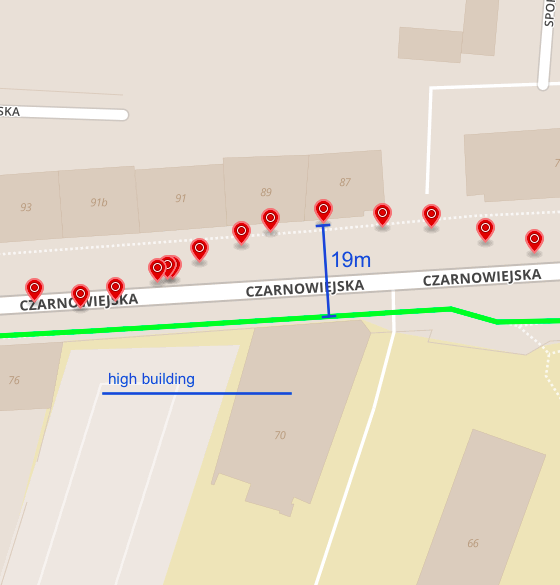
\includegraphics[width=0.9\textwidth]{images/3.png}
    \caption{Green path is the actual path, red pins depict non-filtered readouts. \\ \textit{source: own elaboration}}
    \label{fig:screenexample3}
\end{figure}

\subsection{Example 3: Inaccurate walking readouts} \label{sec:inaccuratereadoutsexample}

Life is not always easy and things like to go badly. As can be seen in the figure \ref{fig:screenexample3}, when approaching high buildings on the south side\footnote{All of the tests were conducted on the north side of the equator.}, readouts became very inaccurate. The readout with largest difference from the actual position was 19 meters, as shown in the figure \ref{fig:screenexample3}. We think this is something that can be solved and we describe proposed solution in the section \ref{sec:futurework}.
